\documentclass[xcolor=usenames,dvipsnames]{beamer}

% ============================================================
% PhD Defense Presentation — Ece Yagman
% Based on Gender Paper 2025 template (Boadilla + serif)
% ============================================================

% THEME + LAYOUT
\mode<presentation>{
  \usetheme{Boadilla}
  \usecolortheme{default}
  \usefonttheme{serif}
  \useoutertheme[compress]{miniframes}
  \setbeamertemplate{navigation symbols}{}
  \setbeamertemplate{footline}[frame number]
}

% FONTS
\usepackage[utf8]{inputenc}
\usepackage[T1]{fontenc}
\AtBeginDocument{\fontencoding{OT1}\selectfont}
\renewcommand{\familydefault}{\rmdefault}

% COLOR PALETTE
\definecolor{HopBlue}{HTML}{1A5C9A}
\definecolor{DarkText}{HTML}{222222}
\definecolor{fadegray}{gray}{0.80}

\setbeamercolor{normal text}{fg=DarkText,bg=white}
\setbeamercolor{structure}{fg=HopBlue}
\setbeamercolor{title}{fg=HopBlue}
\setbeamercolor{frametitle}{fg=HopBlue}
\setbeamercolor{block title}{fg=white,bg=HopBlue}
\setbeamercolor{block body}{bg=HopBlue!5}

% NAV BAR COLORS
\setbeamercolor{section in head/foot}{bg=white, fg=HopBlue}
\setbeamercolor{section in head/foot shaded}{bg=white, fg=DarkText!60}
\setbeamercolor{headline}{bg=HopBlue!12}

% HEADLINE TEMPLATE WITH SECTION NAV
\makeatletter
\setbeamertemplate{headline}{%
  \begin{beamercolorbox}[wd=\paperwidth,ht=5ex,dp=1ex]{headline}%
    \hbox to \paperwidth{%
      \vbox to 4.5ex{%
        \vfil
        \insertsectionnavigationhorizontal{\paperwidth}{}{}
        \vfil
      }%
    }%
  \end{beamercolorbox}%
}
\makeatother

% TITLES
\setbeamerfont{title}{series=\bfseries,size=\LARGE}
\setbeamerfont{frametitle}{series=\bfseries,size=\Large}
\setbeamerfont{section in head/foot}{size=\tiny}

% BULLETS
\usepackage{tikz}
\usetikzlibrary{arrows.meta,positioning}
\setbeamertemplate{itemize item}{%
  \tikz{\draw[fill=HopBlue,draw=HopBlue] (0,0)--(.14,.07)--(0,.14)--cycle;}
}
\setbeamertemplate{itemize subitem}{%
  \tikz{\draw[fill=HopBlue,draw=HopBlue] (0,0)--(.11,.055)--(0,.11)--cycle;}
}

% "PILL" TAGS
\newcommand{\pill}[1]{%
  \tikz[baseline]{\node[
    rounded corners=10pt,
    fill=HopBlue!15,
    inner xsep=6pt, inner ysep=2pt,
    text=HopBlue
  ]{\footnotesize #1};}%
}

% CUSTOM COMMANDS
\newcommand{\fadecolor}[2]{%
  \alt<#1->{#2}{\textcolor{fadegray}{#2}}%
}
\newcommand{\hlcoef}[1]{\textcolor{HopBlue}{\textbf{#1}}}

% AUTOMATIC SECTION DIVIDERS
% \AtBeginSection[]{
%   \begin{frame}[plain]
%     \vspace{2cm}
%     {\LARGE \textbf{\insertsectionhead}}
%     \vspace{0.2cm}
%     {\color{HopBlue}\rule{0.4\linewidth}{2pt}}
%   \end{frame}
% }

% LINKS
\usepackage{hyperref}
\hypersetup{
  colorlinks=true,
  linkcolor=HopBlue,
  citecolor=HopBlue,
  filecolor=HopBlue,
  urlcolor=HopBlue
}

% ---- OTHER PACKAGES ----
\usepackage{dcolumn}
\usepackage{rotating}
\usepackage[table]{xcolor}
\usepackage[english]{babel}
\usepackage{booktabs}
\usepackage{graphicx}
\usepackage{apacite}
\usepackage{natbib}
\usepackage{pifont}
\renewcommand*{\bibfont}{\scriptsize}
\usepackage{appendixnumberbeamer}
\usepackage{threeparttable}
\usepackage{adjustbox}
\usepackage{pdfpages}
\usepackage{siunitx}
\usepackage{wrapfig}
\usepackage{amsmath,amssymb,amsthm}
\newcommand{\sym}[1]{\ifmmode^{#1}\else$^{#1}$\fi}
\newcommand{\MyNumthree}[1]{\num[round-mode=places,round-precision=3]{#1}}
\newcommand{\MyNumtwo}[1]{\num[round-mode=places,round-precision=2]{#1}}
\bibliographystyle{apacite}

\usepackage{totcount}
\regtotcounter{framenumber}

% ============================================================
% TITLE INFO
% ============================================================
\title{Socioemotional Skills in the Classroom:\\
Measurement, Gender Dynamics, and Social Identity}
\author{Ece Yagman}
\institute{Universitat Aut\`onoma de Barcelona \\ PhD Defense}
\date{April 7th, 2026} %TODO: fill in defense date

\titlegraphic{
\includegraphics[width=0.2\textwidth]{figures/Logo.png}}


\newcommand{\grantack}{\tiny
This study has received financial support from grant PID2020-117523GB-I00 funded by\\
MICIU/AEI/10.13039/501100011033
}
\addtobeamertemplate{title page}{}
{%
  \vspace{-1.5em}
  \begin{center}
    \grantack
  \end{center}
}

% ============================================================
\begin{document}
% ============================================================

% ---- TITLE PAGE (slide 1) ----
\begin{frame}[plain]
  \titlepage
\end{frame}

\addtocounter{framenumber}{-1}

% Custom footline: page X / total
\setbeamertemplate{footline}{
  \leavevmode%
  \hbox{%
    \begin{beamercolorbox}[wd=.9\paperwidth,ht=2.5ex,dp=1ex,right]{page number in head/foot}%
      \usebeamerfont{page number in head/foot}%
      \insertframenumber{} / \total{framenumber}\hspace*{2ex}
    \end{beamercolorbox}%
  }%
  \vskip0pt%
}


% %%%%%%%%%%%%%%%%%%%%%%%%%%%%%%%%%%%%%%%%%%%%%%%%%%%%%%%%%%%%
% INTRODUCTION  (slides 2--9)
% %%%%%%%%%%%%%%%%%%%%%%%%%%%%%%%%%%%%%%%%%%%%%%%%%%%%%%%%%%%%
\section{Introduction} 

% ---- Slide 2: The Big Picture ----
\begin{frame}{The Big Picture}
\small
\textbf{Socioemotional skills are central to human capital formation --- yet they remain elusive to define and measure}

\begin{itemize}
    \item Strong predictors of long-term outcomes: educational success, earnings, well-being \citep{Heckman2012-nt}
    \item Distinct from personality traits: SES are malleable, context-dependent competencies that can be developed through instruction
    \item No shared taxonomy --- overlapping labels and frameworks
    \item Gap in \emph{repeated, classroom-embedded} measurement within school systems
\end{itemize}

\vspace{0.3cm}
\textbf{The challenge is especially acute in schools:}
\begin{itemize}
    \item Education systems are increasingly expected to foster SES, not just academics
    \item Daily classroom interactions shape their development
    \item Yet educators lack behavioral anchors and consistent tools for tracking these skills
\end{itemize}
\end{frame}


% ---- Slide 3: This Thesis ----
\begin{frame}{This Thesis}
\small
\textbf{What happens when SEL is embedded into routine classroom instruction?}

\vspace{0.2cm}
The pedagogical program at the center of this thesis, \emph{Pentabilities}, maps broad socioemotional skills into 35 observable behaviors across five domains, and relies on repeated teacher, peer, and self assessments recorded through a digital platform to structure feedback and goal setting.

\vspace{0.3cm}
\textbf{Three chapters provide evidence on three questions:}
\begin{enumerate}
    \item \textbf{Causal effects} of the pedagogy on classroom practices and student outcomes
    \item \textbf{Systematic patterns} in how adolescents evaluate themselves and one another
    \item \textbf{Whether the program narrows} evaluative gaps across gender and national origin
\end{enumerate}
\end{frame}


% ---- Slide 4: Three Chapters ----
\begin{frame}{Three chapters at a glance}
\small
\centering
\begin{tabular}{p{0.8cm} p{4.2cm} p{1.2cm} p{2cm}}
\toprule
Chapter & Question & Sample & Focus \\
\midrule
1 & Does the program work? & T + C & --- \\
2 & Are evaluations gendered? & T only & Gender \\
3 & Can the program reduce in-group bias? & T + C & Gender + Nationality \\
\bottomrule
\end{tabular}
\end{frame}


% ---- Slide 6: The Pedagogical Program ----
\begin{frame}{The Pedagogical Program}
\footnotesize
\begin{columns}[T,onlytextwidth]
  \begin{column}{0.68\textwidth}
    \begin{itemize}
      \item \textbf{Context:} 40 public secondary schools in Catalonia, Spain (2022--2023)
      \item 148 classrooms, 129 teachers, 2,451 students aged 12--17
      \item Schools serving predominantly disadvantaged communities (stratified: 50\% medium, 50\% high complexity)
      \item \textbf{Program} (developed by Pentabilities SL):
      \begin{itemize}\footnotesize
        \item Curriculum-embedded SEL: integrated into regular instruction, not a separate class
        \item Built on observable behaviors reflecting latent SES \citep{Heckman2012-nt, Jackson2018-ho}
        \item 35 observable behaviors organized into 5 domains
        \item Cooperative group work with rotating team composition
        \item Digital 360$^{\circ}$ assessment: teachers, peers, and students record ratings via app
        \item Evidence-based feedback: periodic reports guide goal-setting and reflection
      \end{itemize}
    \end{itemize}
  \end{column}
  \begin{column}{0.30\textwidth}
    \centering
    \includegraphics[width=\linewidth]{figures/PB 5-factor.png}
  \end{column}
\end{columns}
\vspace{0.2cm}
\footnotesize\textbf{Key design feature:} Pedagogy and measurement are intertwined --- the same system that supports skill development also generates the data
\end{frame}


% ---- Slide 7: Five Domains ----
\begin{frame}{Five Domains}
%TODO: Reuse the colorful 5-domain card from existing slides
%\includegraphics[width=\linewidth]{figures/PB 5-factor.png}
\begin{center}
\small
\begin{tabular}{lp{8cm}}
\toprule
\textbf{Domain} & \textbf{Example behaviors} \\
\midrule
Responsibility & Works consistently, perseveres through difficulties, respects rules \\
Autonomy \& Initiative & Brings up ideas, works with determination, takes active role \\
Cooperation & Listens to others, encourages participation, facilitates conflict resolution \\
Emotional Management & Remains calm under pressure, controls emotions, accepts mistakes \\
Thinking Abilities & Makes good reflections, asks good questions, proposes strategies \\
\bottomrule
\end{tabular}
\end{center}

\vspace{0.3cm}
Each behavior scored on 1--5 Likert scale by multiple raters
\end{frame}


% ---- Slide 8: The RCT Design ----
\begin{frame}{The RCT Design}
\small
\textbf{Randomization:} Grade level within schools (cluster)
\begin{itemize}
    \item Stratified by school disadvantage level
    \item Treatment: 69 classrooms (1,164 students) --- Control: 72 classrooms (1,200 students)
    \item Balanced on all observable student, family, and school characteristics
\end{itemize}

\vspace{0.3cm}
\textbf{Three measurement instruments:}

\footnotesize
\begin{tabular}{lllll}
\toprule
Instrument & Setting & Raters & T/C & Used in \\
\midrule
\textbf{CO} & Regular class, repeated & Self, Peer, Tch, EO & T only & Ch.1, 2 \\
\textbf{FA} & Lab-in-the-field, random groups & Self, Peer, EO & T + C & Ch.2, 3 \\
\textbf{BESSI} & Endline survey (Soto et al., 2022) & Self, Peer, Tch & T + C & Ch.2, 3 \\
\bottomrule
\end{tabular}
\end{frame}


% ---- Slide 9: Data Architecture ----
\begin{frame}{Data Architecture: 360$^{\circ}$ Measurement}
\small
%TODO: Insert diagram showing the 360° measurement system
%\includegraphics[width=0.8\textwidth]{figures/data_architecture.png}

For each student, we observe:
\begin{itemize}
    \item How they rate \textbf{themselves} (SELF)
    \item How \textbf{peers} rate them (CO/PEER)
    \item How \textbf{teachers} rate them (TCH)
    \item How \textbf{external observers} rate them (EO)
\end{itemize}

\vspace{0.3cm}
$\Rightarrow$ This multi-rater design lets us:
\begin{itemize}
    \item Benchmark self-perception against ability (teacher, EO)
    \item Isolate who drives evaluation gaps (student gender $\times$ peer gender)
    \item Separate skill differences from perception differences
\end{itemize}
\end{frame}


% %%%%%%%%%%%%%%%%%%%%%%%%%%%%%%%%%%%%%%%%%%%%%%%%%%%%%%%%%%%%
% CHAPTER 1: TREATMENT EFFECTS  (slides 10--14 + bridge 16)
% %%%%%%%%%%%%%%%%%%%%%%%%%%%%%%%%%%%%%%%%%%%%%%%%%%%%%%%%%%%%
\section{Chapter 1}
% NOTE: \AtBeginSection auto-generates the chapter divider slide

% ---- Slide 11: Empirical Strategy ----
\begin{frame}{Empirical Strategy}
\small
\textbf{Intent-to-treat (ITT), ANCOVA specification:}
\begin{equation*}
Y_{i,el} = \alpha + \alpha_1 \cdot \text{Treated}_i + \mathbf{X}_{i,bl}' \boldsymbol{\beta} + \text{Strata\_FE} + \varepsilon_i
\end{equation*}

\begin{itemize}
    \item Outcome $Y$ measured at endline; baseline controls $\mathbf{X}_{bl}$ when available
    \item Strata fixed effects (randomization block)
    \item Standard errors clustered at school-grade level
\end{itemize}

\vspace{0.3cm}
\textbf{Outcomes:}
\begin{enumerate}
    \item Classroom environment (teacher time use, student perceptions)
    \item Student socioemotional skills (BESSI, FA, surveys)
    \item Academic outcomes (GPA, attendance)
\end{enumerate}

\vspace{0.3cm}
\footnotesize
\textit{Note: A substantially updated version --- with coauthors Calsamiglia, De Giorgi, Navarro-Sola, and Salvati --- was presented at CESifo 2025. The main advance: the program's effects on classroom processes are concentrated among disadvantaged students.}
\end{frame}


% ---- Slide 12: Classroom Environment ----
\begin{frame}{Result: Classroom Environment Transforms}
\small
\textbf{Teachers reallocate time:}
\begin{itemize}
    \item 42\% reduction in time managing discipline during class
    \item 26\% reduction outside classroom
    \item Time shifts toward student autonomy and peer exchange
\end{itemize}

\vspace{0.3cm}
\textbf{Students notice the change:}
\begin{itemize}
    \item Treated students rate teachers +0.13 to +0.20 SD higher on composite perception score
    \item Higher ratings on classroom atmosphere and feedback quality items
\end{itemize}

\vspace{0.5cm}
\textit{The program reorganizes how classrooms function --- changing the structure of interactions and the evaluative environment}
\end{frame}


% ---- Slide 13: Student Outcomes ----
\begin{frame}{Result: Student Outcomes}
\small
\textbf{No short-run effects on:}
\begin{itemize}
    \item Socioemotional skills (behavioral task, survey assessments)
    \item Academic achievement (GPA)
    \item Attendance
\end{itemize}

\vspace{1cm}
%TODO: Insert treatment effect estimates table or figure
%\includegraphics[width=0.7\textwidth]{figures/ch1_outcomes.png}
\end{frame}


% ---- Slide 14: The Evaluative Environment ----
\begin{frame}{The Evaluative Environment}
\small
The program introduces cooperative group work, behavior-anchored rubrics, and repeated multi-rater assessment. The first thing that changes is the \textbf{informational environment}:

\begin{itemize}
    \item Students evaluate each other systematically, using shared criteria
    \item The classroom becomes a space where perceptions of competence are actively constructed
    \item The same infrastructure that supports skill development generates the data that reveals how students perceive themselves and each other
\end{itemize}

\vspace{0.5cm}
\textit{If the classroom environment has changed, the question becomes: for whom has it changed, and what patterns emerge in how students use these new evaluative tools?}

%TODO: Insert Theory of Change flowchart
%\includegraphics[width=0.8\textwidth]{figures/theory_of_change.png}
\end{frame}


% ---- Bridge 1 (slide 16) ----
\begin{frame}{From Average Effects to Gender Dynamics}
\small
\textbf{Chapter 1 shows the program changes how classrooms operate.}

\vspace{0.3cm}
But the 360$^{\circ}$ measurement system reveals something else: when students evaluate themselves and each other, systematic patterns emerge that follow gender lines.

\vspace{0.5cm}
\textbf{Next:} Do self- and peer-perceptions of SES differ for female vs.\ male adolescents?
\end{frame}


% %%%%%%%%%%%%%%%%%%%%%%%%%%%%%%%%%%%%%%%%%%%%%%%%%%%%%%%%%%%%
% CHAPTER 2: GENDER GAPS  (slides 17--28 + bridge 29)
% %%%%%%%%%%%%%%%%%%%%%%%%%%%%%%%%%%%%%%%%%%%%%%%%%%%%%%%%%%%%
\section{Chapter 2}

% ---- Slide 18: Why Adolescence? ----
\begin{frame}{Why Adolescence?}
\small
\begin{itemize}
    \item Ages 12--16: high neuroplasticity, self-beliefs and aspirations are particularly malleable \citep{Steinberg2014-pe}
    \item \textbf{Self-identity formation:} Who am I? What am I good at? Where do I fit in?
    \item \textbf{Peer-influence peaks:} Students look to classmates for cues --- who is good at what?
    \item Gendered norms around ``girls do well'' vs.\ ``boys do well'' solidify during these years
\end{itemize}

\vspace{0.5cm}
\textit{Early differences in self-beliefs or peer recognition can shape confidence and aspirations for years to come}
\end{frame}


% ---- Slide 19: Two Research Questions ----
\begin{frame}{Two Research Questions}
\small
\textbf{Question 1 --- Self-evaluation:}\\
Do female students rate their own SES differently from male students, conditional on ability?

\vspace{0.3cm}
\textbf{Question 2 --- Peer evaluation:}\\
Is there a systematic gender pattern in how peers evaluate each other's SES?

\vspace{0.5cm}
\textbf{Why this matters:}
\begin{itemize}
    \item Evaluations are not just measures of skill --- they shape beliefs, motivation, and the feedback environment
    \item Gendered patterns that form in adolescence can influence later educational and labor market choices
\end{itemize}
\end{frame}


% ---- Slide 20: Empirical Strategy — Self-Evaluation ----
\begin{frame}{Empirical Strategy: Self-Evaluation}
\small
\begin{block}{Specification (CO, BESSI, FA)}
\vspace{-0.2cm}
\begin{equation*}
\text{Self}_{is} = \alpha
   + \boldsymbol{\gamma_1} \mathbf{Female}_i
   + \gamma_2 \, \text{Teacher}_{is}
   + \gamma_3 \, \overline{\text{Peer}}_{is}
   + \mathbf{X}'_i \boldsymbol{\beta}
   + \alpha_c
   + \varepsilon_{is}
\end{equation*}
\end{block}

\begin{itemize}
    \item Conditioning on teacher and peer scores = proxying for actual ability
    \item $\gamma_1$ captures: do females self-rate differently, \emph{holding ability constant}?
    \item Estimated separately for CO (classroom observations), BESSI (survey), and FA (lab task)
    \item $\alpha_c$: classroom fixed effects
\end{itemize}
\end{frame}


% ---- Slide 21: Result — Females Underrate Themselves ----
\begin{frame}{Females Underrate Themselves}
\small
\textbf{Conditional on ability (z-scored, classroom FE):}

\vspace{0.2cm}
\footnotesize
\begin{center}
\begin{tabular}{llrl}
\toprule
Dataset & Domain & Female coeff. & Sig. \\
\midrule
CO & Emotional Management & $-$0.302 & *** \\
CO & Thinking Abilities & $-$0.239 & *** \\
BESSI & Emotional Management & $-$0.467 & *** \\
BESSI & Social Engagement & $-$0.309 & *** \\
BESSI & Self Management & $-$0.229 & *** \\
BESSI & Cooperation & $-$0.162 & *** \\
FA & Emotional Management & negative & * \\
FA & Thinking Abilities & negative & * \\
\bottomrule
\end{tabular}
\end{center}

\vspace{0.2cm}
\small
\textit{Consistent across all three instruments: girls discount their own SES, especially in Emotional Management and Thinking}

\vspace{0.2cm}
\hyperlink{slide:self_full}{\beamergotobutton{Full Tables}}
\end{frame}


% ---- Slide 22: Empirical Strategy — Peer Evaluations ----
\begin{frame}{Empirical Strategy: Peer Evaluations}
\small
\begin{block}{Main specification (CO, treated schools only)}
\vspace{-0.2cm}
\begin{eqnarray}
    y_{ijs} &=& \beta_0
    + \beta_1 \, \text{StuFem}_{i}
    + \beta_2 \, \text{PeerFem}_{j}
    + \boldsymbol{\beta_3} \, (\mathbf{StuFem \times PeerFem})_{ij}
 \nonumber \\
    &&
    + \text{Controls}
    + \alpha_c
    + \varepsilon_{ijs}
    \nonumber
\end{eqnarray}
\end{block}

\begin{itemize}
    \item Clustered SE at student level
    \item Controls: teacher score, peer's self-score, student background
    \item Reference group: male student rated by male peer
\end{itemize}

\vspace{0.3cm}
\textbf{Key coefficient:} \hlcoef{$\beta_3$} --- the additional effect when both student and peer are female
\end{frame}


% ---- Slide 23: The Female-Female Premium ----
\begin{frame}{The Female-Female Premium}
\label{slide:ff_premium}

%TODO: Replace table with coefficient plot figure once generated
%\includegraphics[width=0.8\textwidth]{figures/coefplot_ff_premium.png}

\footnotesize
\begin{center}
\begin{tabular}{lccc}
\toprule
Domain & $\beta_1$ (Fem Student) & $\beta_2$ (Fem Peer) & \hlcoef{$\beta_3$ (FF Interaction)} \\
\midrule
Autonomy & $+$0.04 & $-$0.20\sym{***} & \hlcoef{$+$0.43\sym{***}} \\
Cooperation & $+$0.10\sym{*} & $-$0.21\sym{***} & \hlcoef{$+$0.32\sym{***}} \\
Responsibility & $+$0.23\sym{***} & $-$0.19\sym{***} & \hlcoef{$+$0.24\sym{***}} \\
Emotional Mngt & $+$0.03 & $-$0.23\sym{***} & \hlcoef{$+$0.27\sym{***}} \\
Thinking & $-$0.00 & $-$0.33\sym{***} & \hlcoef{$+$0.37\sym{***}} \\
\bottomrule
\end{tabular}
\end{center}

\vspace{0.1cm}
\scriptsize $N \approx$ 30,000+ peer evaluations across $\sim$911 students, 88 classrooms

\vspace{0.2cm}
\small
\hyperlink{slide:peer_full}{\beamergotobutton{Full Tables}}
\hyperlink{slide:gender_int}{\beamergotobutton{Net Effect}}
\end{frame}


% ---- Slide 24: Interpreting the Premium ----
\begin{frame}{Interpreting the Premium}
\small
\textbf{Three clear patterns:}

\vspace{0.3cm}
\begin{enumerate}
    \item<1-> \fadecolor{1}{\textbf{Male peers are gender-neutral:} $\beta_1$ is small/insignificant $\rightarrow$ males don't rate female students differently from male students}
    \vspace{0.2cm}
    \item<2-> \fadecolor{2}{\textbf{Female peers are strict toward males:} $\beta_2$ is negative and significant in all domains $\rightarrow$ female peers give lower scores when rating male students}
    \vspace{0.2cm}
    \item<3-> \fadecolor{3}{\textbf{Female-female premium:} $\beta_3$ is large and positive $\rightarrow$ when a female peer rates a female student, there is an additional +0.24 to +0.43 SD boost}
\end{enumerate}

\vspace{0.3cm}
\onslide<3->{%
\textbf{Net female-female effect ($\beta_1 + \beta_3$):} +0.21 to +0.37 SD above the male-male baseline

\vspace{0.2cm}
\textit{This is concentrated in WHO is doing the rating, not in WHO is being rated}
}
\end{frame}


% ---- Slide 25: Robustness ----
\begin{frame}{Robustness: Consistent Across Settings}
\small
\textbf{Lab-in-the-field (FA):}
\begin{itemize}
    \item Random group assignment $\rightarrow$ eliminates friendship confound
    \item Same directional pattern, attenuated magnitudes
    \item FF premium: +0.17 to +0.27 SD
\end{itemize}

\vspace{0.2cm}
\textbf{BESSI endline survey:}
\begin{itemize}
    \item Validated 360$^{\circ}$ instrument, all schools (T + C)
    \item FF premium: +0.21 to +0.37 SD across all 5 BESSI domains
\end{itemize}

\vspace{0.2cm}
\textbf{External observer ratings:} Confirm patterns are not driven by teacher bias or classroom dynamics

\vspace{0.3cm}
\textit{Robust across evaluators, settings, and measurement methods}

\vspace{0.2cm}
\hyperlink{slide:rob_eo}{\beamergotobutton{EO}} \quad
\hyperlink{slide:rob_fa}{\beamergotobutton{FA}} \quad
\hyperlink{slide:rob_bessi}{\beamergotobutton{BESSI}}
\end{frame}


% ---- Slide 26: The Paradox ----
\begin{frame}{The Paradox}
\small

%TODO: Insert side-by-side paradox visual
%\includegraphics[width=0.8\textwidth]{figures/paradox_visual.png}

\begin{columns}[T]
\begin{column}{0.48\textwidth}
\onslide<1->{%
\textbf{\textcolor{HopBlue}{How female students see themselves:}}
\begin{itemize}
    \item Rate themselves lower in Emotional Mngt ($-$0.30 to $-$0.47 SD)
    \item Rate themselves lower in Thinking ($-$0.24 SD)
    \item Consistent with stereotype-congruent domains \citep{Exley2022-tt}
\end{itemize}
}
\end{column}

\begin{column}{0.48\textwidth}
\onslide<2->{%
\textbf{\textcolor{HopBlue}{How their peers see them:}}
\begin{itemize}
    \item Female peers rate female students \emph{higher} across ALL domains (+0.21 to +0.37 SD)
    \item The very skills girls doubt in themselves are the ones peers recognize most
\end{itemize}
}
\end{column}
\end{columns}

\vspace{0.5cm}
\onslide<2->{%
\textit{Girls do not project their self-discount onto female classmates --- they recognize and endorse others' strengths while doubting their own}
}
\end{frame}


% ---- Slide 27: Policy Relevance ----
\begin{frame}{Policy Relevance}
\small
\textbf{Targeted interventions to reduce misperceptions:}
\begin{itemize}
    \item Show students the gap between their own assessment and what peers and teachers see
    \item Make blind spots visible: where self-ratings diverge most from external benchmarks
    \item Structured feedback sessions that use the 360$^{\circ}$ data to calibrate self-perception
\end{itemize}

\vspace{0.3cm}
\textbf{Discussions around gender norms and stereotypes:}
\begin{itemize}
    \item SES respond to well-structured school-based programs that address misperceptions \citep{Alan2025-jr}
    \item Educational discussion groups around gender norms among adolescents can reduce misperceptions \citep{Matavelli2025-gh}, with effects that persist beyond the short run \citep{Dhar2022-cn}
\end{itemize}

\vspace{0.3cm}
\footnotesize
\textit{The program was not designed as a debiasing tool, but its evaluative infrastructure could be leveraged for targeted interventions}
\end{frame}


% ---- Slide 28: Chapter 2 Takeaway ----
\begin{frame}{Chapter 2: Takeaway}
\small
\textbf{Two robust findings:}

\vspace{0.2cm}
\begin{enumerate}
    \item \textbf{Self-evaluation:} Females underrate their SES conditional on ability, especially in Emotional Management and Thinking --- domains where gender stereotypes are strongest
    \vspace{0.2cm}
    \item \textbf{Peer evaluation:} A substantial female-female premium exists across all domains, driven by female peers' evaluative patterns
\end{enumerate}

\vspace{0.3cm}
\textbf{These matter because:}
\begin{itemize}
    \item Evaluations shape the feedback environment students experience
    \item Gendered patterns in adolescence can become self-reinforcing
    \item They point to a feature of the evaluative system, not just individual psychology
\end{itemize}

\vspace{0.3cm}
\textit{Can the program --- designed for skill-building --- reshape these patterns?}
\end{frame}


% ---- Bridge 2 (slide 29) ----
\begin{frame}{From Documenting Patterns to Testing Solutions}
\small
\textbf{Chapter 2 documented systematic identity-based patterns in evaluations.}

\vspace{0.3cm}
The program in Chapter 1 was not designed as a debiasing intervention --- it targets skill development through cooperative work and structured feedback.

\vspace{0.3cm}
\textbf{But its features} --- rotating groups, cross-group interaction, behavior-anchored criteria --- \textbf{align with conditions known to reduce in-group bias} (Allport, 1954; Pettigrew \& Tropp, 2006).

\vspace{0.5cm}
\textbf{Next:} Can we detect causal debiasing spillovers?
\end{frame}


% %%%%%%%%%%%%%%%%%%%%%%%%%%%%%%%%%%%%%%%%%%%%%%%%%%%%%%%%%%%%
% CHAPTER 3: IN-GROUP FAVORITISM  (slides 30--39)
% %%%%%%%%%%%%%%%%%%%%%%%%%%%%%%%%%%%%%%%%%%%%%%%%%%%%%%%%%%%%
\section{Chapter 3}

% ---- Slide 31: Research Questions + Design ----
\begin{frame}{Research Questions and Design}
\small
\textbf{Two questions:}
\begin{enumerate}
    \item Do adolescents display own-group favoritism in peer assessments of SES? (Gender + Nationality)
    \item Can the Pentabilities program attenuate these in-group biases?
\end{enumerate}

\vspace{0.3cm}
\textbf{Design advantage over Chapter 2:}
\begin{itemize}
    \item Full treatment/control comparison (randomized rollout)
    \item Two complementary instruments:
    \begin{itemize}
        \item \textbf{FA (lab-in-the-field):} task-based, random groups, behavior-grounded ratings
        \item \textbf{BESSI (survey):} reputation-based, broader perceived capacity
    \end{itemize}
\end{itemize}

\vspace{0.2cm}
\textit{Comparing both reveals what changes first}
\end{frame}


% ---- Slide 32: Empirical Strategy ----
\begin{frame}{Empirical Strategy: Triple Interaction}
\small
\begin{eqnarray}
y_{ijgs} &=& \alpha
+ \beta_1\,\text{StuFem}
+ \beta_2\,\text{PeerFem}
+ \beta_3\,(\text{StuFem} \times \text{PeerFem})
\nonumber \\
&&
+ \beta_4\,\text{Treated}
+ \beta_5\,(\text{StuFem} \times \text{Treated})
+ \beta_6\,(\text{PeerFem} \times \text{Treated})
\nonumber \\
&&
+ \boldsymbol{\beta_7}\,(\mathbf{StuFem \times PeerFem \times Treated})
\nonumber \\
&&
+ \text{360$^{\circ}$ score controls}
+ \text{Background controls}
+ \text{School\_FE}
+ \varepsilon
\nonumber
\end{eqnarray}

\vspace{0.2cm}
\begin{itemize}
    \item \hlcoef{$\beta_3$}: in-group premium in \textbf{control} classrooms
    \item \hlcoef{$\beta_7$}: \textbf{treatment effect} on the in-group premium (key parameter)
    \item SE clustered at school-grade (randomization) level
\end{itemize}

\vspace{0.2cm}
Same framework for nationality: replace gender indicators with born-in-Spain indicators
\end{frame}


% ---- Slide 33: Gender In-Group (Lab Task) ----
\begin{frame}{Gender In-Group Bias: Lab Task (FA)}
\small
\textbf{In control classrooms:} FF premium replicates: +0.22 to +0.35 SD across all 5 domains (all significant)

\vspace{0.2cm}
\textbf{Treatment effect (triple interaction $\beta_7$):}

\footnotesize
\begin{center}
\begin{tabular}{lcc}
\toprule
Domain & FF Premium (Control) & Treatment Effect \\
\midrule
Autonomy & $+$0.22\sym{**} & $-$0.10 \\
\textbf{Cooperation} & $+$\textbf{0.33}\sym{***} & $-$\textbf{0.18}\sym{*} \\
Responsibility & $+$0.35\sym{***} & $-$0.20 \\
Emotion & $+$0.23\sym{***} & $-$0.13 \\
Thinking & $+$0.25\sym{***} & $-$0.04 \\
\bottomrule
\end{tabular}
\end{center}

\vspace{0.2cm}
\small
\textit{Treatment compresses the FF premium, significantly in Cooperation ($\sim$1/5 SD reduction)}
\end{frame}


% ---- Slide 34: Gender In-Group (BESSI) ----
\begin{frame}{Gender In-Group Bias: BESSI Survey}
\small
\textbf{In control classrooms:}
\begin{itemize}
    \item FF premium: +0.29 to +0.43 SD (all significant) --- even larger than FA
\end{itemize}

\vspace{0.3cm}
\textbf{Treatment effect:}
\begin{itemize}
    \item Negative in 4/5 domains (magnitudes $-$0.02 to $-$0.16 SD)
    \item \textbf{Not statistically significant}
\end{itemize}

\vspace{0.5cm}
\textit{Same direction as FA but less precise --- reputation-based beliefs are stickier than task-based ratings}
\end{frame}


% ---- Slide 35: Nationality ----
\begin{frame}{Nationality In-Group Bias}
\small
\textbf{National origin (Spain-born vs.\ foreign-born):}

\vspace{0.3cm}
\textbf{In control classrooms (FA):}
\begin{itemize}
    \item Suggestive Spain-origin in-group premium in Autonomy and Cooperation (+0.20--0.28)
    \item Not statistically significant (larger SEs)
\end{itemize}

\vspace{0.3cm}
\textbf{Treatment effect:}
\begin{itemize}
    \item Negative in Cooperation (pointing to dampening)
    \item Imprecisely estimated in full sample
\end{itemize}

\vspace{0.5cm}
\textbf{But in low-diversity classrooms\ldots}
\end{frame}


% ---- Slide 36: Classroom Diversity Heterogeneity ----
\begin{frame}{Key Heterogeneity: Classroom Diversity}
\small

%TODO: Insert split coefficient plot by diversity level
%\includegraphics[width=0.8\textwidth]{figures/diversity_heterogeneity.png}

\begin{columns}[T]
\begin{column}{0.48\textwidth}
\textbf{\textcolor{HopBlue}{Low-diversity classrooms:}}
\begin{itemize}
    \item Baseline in-group premiums are substantially larger
    \item \textbf{The program compresses them across nearly all domains}
    \item Where structured cross-group contact is most novel
\end{itemize}
\end{column}

\begin{column}{0.48\textwidth}
\textbf{\textcolor{HopBlue}{High-diversity classrooms:}}
\begin{itemize}
    \item Smaller baseline premiums (more natural cross-group exposure)
    \item Treatment effects muted
\end{itemize}
\end{column}
\end{columns}

\vspace{0.5cm}
\textit{Context matters: the intervention has highest returns where out-group exposure is most limited}
\end{frame}


% ---- Slide 37: FA vs BESSI ----
\begin{frame}{FA vs.\ BESSI: What Changes First?}
\small

%TODO: Insert two-panel comparison visual
%\includegraphics[width=0.8\textwidth]{figures/fa_vs_bessi.png}

\footnotesize
\begin{center}
\begin{tabular}{lll}
\toprule
Feature & FA (Lab Task) & BESSI (Survey) \\
\midrule
Basis & Specific, shared interaction & General reputation \\
Rating anchor & Recent observed behavior & Accumulated impressions \\
Treatment response & Faster (sig.\ in Cooperation) & Slower (same direction, n.s.) \\
\bottomrule
\end{tabular}
\end{center}

\vspace{0.3cm}
\small
\textbf{Interpretation:}
\begin{itemize}
    \item Task-based ratings respond more quickly because they are anchored in direct behavioral evidence
    \item Survey-based ratings lean on broader beliefs that are slower to update
    \item The program's debiasing spillovers show up first where evaluation is closest to behavior
\end{itemize}

\vspace{0.2cm}
\textit{The program increases behavior-relevant information and makes evaluation criteria more explicit}
\end{frame}


% ---- Slide 38: Two Mechanisms ----
\begin{frame}{Two Mechanisms}
\small
\textbf{1. Cooperative contact}
\begin{itemize}
    \item Rotating group composition expands who students interact with
    \item Working together toward shared goals $\rightarrow$ conditions of Allport's contact hypothesis
    \item The program creates structured, repeated, equal-status intergroup interaction
\end{itemize}

\vspace{0.3cm}
\textbf{2. Disciplined evaluation}
\begin{itemize}
    \item Behavior-anchored rubrics give students concrete criteria
    \item Ratings become formative data discussed in feedback sessions
    \item Students are trained to evaluate based on observable behaviors rather than priors or stereotypes
\end{itemize}

\vspace{0.3cm}
\textit{Together: the program changes both WHO you interact with and HOW you evaluate them}
\end{frame}


% ---- Slide 39: Chapter 3 Takeaway ----
\begin{frame}{Chapter 3: Takeaway}
\small
\textbf{Main contribution:} A pedagogy designed for skill-building --- not debiasing --- can reduce in-group favoritism in peer evaluations.

\vspace{0.3cm}
\textbf{Three key results:}
\begin{enumerate}
    \item Gender: treatment compresses FF premium in task-based settings (especially Cooperation)
    \item Nationality: treatment effects emerge in low-diversity classrooms where cross-group contact is most constrained
    \item FA vs.\ BESSI divergence: behavioral ratings update faster than reputational beliefs
\end{enumerate}

\vspace{0.5cm}
\textit{Routine classroom pedagogy can reshape the informational environment of evaluation}
\end{frame}


% %%%%%%%%%%%%%%%%%%%%%%%%%%%%%%%%%%%%%%%%%%%%%%%%%%%%%%%%%%%%
% CONCLUSION  (slides 40--46)
% %%%%%%%%%%%%%%%%%%%%%%%%%%%%%%%%%%%%%%%%%%%%%%%%%%%%%%%%%%%%
\section{Conclusion}

% ---- Slide 40: Thesis Summary ----
\begin{frame}{Thesis Summary}
\small

%TODO: Insert three-row architecture diagram
%\includegraphics[width=0.8\textwidth]{figures/thesis_summary.png}

\begin{center}
\footnotesize
\begin{tabular}{clp{6.5cm}}
\toprule
Ch. & Question & Finding \\
\midrule
\textbf{1} & Does the program work? & Reshapes classroom processes; skill effects need longer horizon \\
\textbf{2} & Are evaluations gendered? & Female self-underrating ($-$0.24 to $-$0.47 SD) + FF peer premium (+0.21 to +0.43 SD) \\
\textbf{3} & Can the program reduce bias? & Yes --- compresses in-group premiums, especially task-based ratings in Cooperation \\
\bottomrule
\end{tabular}
\end{center}

\vspace{0.3cm}
\small
\textbf{Unifying thread:} The Pentabilities framework generates an evaluative environment that is both a tool for skill development and a window into how identities shape perceptions. The program can shift both.
\end{frame}


% ---- Slide 41: Contributions ----
\begin{frame}{Contributions}
\small
\textbf{1. Measurement contribution:}
\begin{itemize}
    \item First multi-rater, behavior-based evidence on gendered SES perceptions in adolescence
    \item The 360$^{\circ}$ design allows benchmarking self-perception against ability proxies from multiple raters
\end{itemize}

\vspace{0.2cm}
\textbf{2. Empirical contribution:}
\begin{itemize}
    \item Documents a robust female-female premium in SES peer evaluations (new to the literature)
    \item Establishes that female self-underrating extends to socioemotional domains, not just academic/competitive tasks \citep{Exley2022-tt}
\end{itemize}

\vspace{0.2cm}
\textbf{3. Policy contribution:}
\begin{itemize}
    \item Causal evidence that routine cooperative pedagogy can reduce in-group favoritism
    \item Advances the contact hypothesis literature with a scalable, curriculum-embedded design (vs.\ one-off interventions)
\end{itemize}
\end{frame}


% ---- Slide 42: Policy Implications ----
\begin{frame}{Policy Implications}
\small
\textbf{1. Feedback design can address self-underrating}
\begin{itemize}
    \item Girls receive favorable evaluations from peers but discount their own abilities
    \item Structured feedback showing self vs.\ peer scores could help calibrate self-perception
\end{itemize}

\vspace{0.2cm}
\textbf{2. Context matters for implementation}
\begin{itemize}
    \item Low-diversity classrooms benefit most from structured cooperation
    \item SEL should be attentive to classroom composition --- one-size-fits-all is insufficient
\end{itemize}

\vspace{0.2cm}
\textbf{3. Evaluation horizon matters}
\begin{itemize}
    \item Process measures change first (classroom routines, evaluative norms)
    \item Skill and academic effects may follow with longer exposure
    \item Accountability for SEL should incorporate process measures, not rely exclusively on short-run test scores
\end{itemize}
\end{frame}


% ---- Slide 43: Limitations ----
\begin{frame}{Limitations}
\small
\begin{itemize}
    \item \textbf{Short evaluation window:} One school year (6 months of implementation) --- longer-run effects unmeasured
    \vspace{0.2cm}
    \item \textbf{CO data is treatment-only} in Chapter 2 --- cannot test treatment effects on gender gap within CO
    \vspace{0.2cm}
    \item \textbf{Power for triple interactions:} Some Chapter 3 results are suggestive rather than definitive
    \vspace{0.2cm}
    \item \textbf{Generalizability:} Catalan public secondary schools serving disadvantaged communities --- external validity to other contexts requires further study
    \vspace{0.2cm}
    \item \textbf{Self-report measures:} BESSI and some CO components rely on subjective assessments
\end{itemize}
\end{frame}


% ---- Slide 44: Future Work ----
\begin{frame}{Future Work}
\small
\textbf{Long-run follow-up:}
\begin{itemize}
    \item Linking participants to administrative records $\rightarrow$ track educational trajectories, labor market outcomes, health proxies for up to 8 years
    \item Test whether early self-perception gaps predict later sorting into tracks, fields of study, and jobs
\end{itemize}

\vspace{0.3cm}
\textbf{Deeper mechanism work:}
\begin{itemize}
    \item Whether a pedagogy targeting the evaluation environment in early adolescence attenuates downstream gender gradients
    \item Sharper heterogeneity tests: impacts concentrated among students facing greater disadvantage?
\end{itemize}
\end{frame}


% ---- Slide 45: Closing Message ----
\begin{frame}{}
\large
\textbf{Schools are not just places where skills are taught --- they are environments where students form self-beliefs and evaluate their peers.}

\vspace{0.5cm}
\normalsize
These evaluations carry systematic patterns tied to gender and social identity, patterns that emerge early and can compound over time.

\vspace{0.5cm}
\textbf{This thesis shows that a well-designed classroom pedagogy can begin to shift both the processes and the perceptions --- creating a fairer informational environment for all students.}
\end{frame}


% ---- Slide 46: Thank You ----
\begin{frame}[plain]
\vfill
\begin{center}
{\LARGE \textbf{Thank you / Gr\`acies / Gracias}}

\vspace{1cm}
Ece Yagman \\
\texttt{[email]} \\ %TODO: fill in email
Universitat Aut\`onoma de Barcelona
\end{center}
\vfill
\end{frame}


% %%%%%%%%%%%%%%%%%%%%%%%%%%%%%%%%%%%%%%%%%%%%%%%%%%%%%%%%%%%%
% APPENDIX / BACKUP SLIDES
% %%%%%%%%%%%%%%%%%%%%%%%%%%%%%%%%%%%%%%%%%%%%%%%%%%%%%%%%%%%%
\appendix

\begin{frame}[allowframebreaks]{References}
\def\newblock{}
\bibliography{paperpile}
\end{frame}


\section*{Backup}

% ---- Econometric Specification Reference ----
\begin{frame}{Econometric Specification Reference}
\label{slide:gender_int}
\footnotesize
\textbf{Peer-evaluation regression:}
\[
y_{ijs} = \beta_0
+ \beta_1\,\text{StuFem}_i
+ \beta_2\,\text{PeerFem}_j
+ \beta_3\,(\text{StuFem} \times \text{PeerFem})_{ij}
+ \mathbf{X}'\gamma
+ \alpha_c
+ \varepsilon_{ij}
\]

\vspace{0.2cm}
\begin{tabular}{lll}
\toprule
Coefficient & Comparison & Interpretation \\
\midrule
$\beta_0$ & M student, M peer & Baseline (reference) \\
$\beta_1$ & F stu, M peer vs.\ M stu, M peer & Male peers neutral ($\approx 0$) \\
$\beta_2$ & M stu, F peer vs.\ M stu, M peer & Female peers strict (negative) \\
$\beta_3$ & Interaction (F$\times$F) & \textbf{Premium} (positive) \\
$\beta_1 + \beta_3$ & F stu, F peer vs.\ M stu, F peer & FF premium (+0.19--0.37 SD) \\
\bottomrule
\end{tabular}

\vspace{0.2cm}
\textbf{Controls:} 360$^{\circ}$ scores, student and peer background.
\textbf{FE:} Classroom.
\textbf{Clustering:} Student.
\end{frame}


% ---- Self-Evaluation Full Tables ----
\begin{frame}{Self-Evaluation: Full Tables}
\label{slide:self_full}

\begin{table}[htp]
\centering
\resizebox{0.95\textwidth}{!}{
\begin{threeparttable}
\caption{Self-Assigned Score: All 5 dimensions}
\label{tab:self_compact}
\begin{tabular}{lccccc}
\toprule
 & Autonomy & Cooperation & Responsibility & Emotion  & Thinking \\
\midrule
Female Student & -0.141* & -0.101 & -0.085 & -0.302*** & -0.239*** \\
 & (0.081) & (0.078) & (0.074) & (0.090) & (0.090) \\
Teacher Score & 0.177*** & 0.117** & 0.137*** & 0.087 & 0.042 \\
 & (0.061) & (0.058) & (0.053) & (0.058) & (0.066) \\
Average Peer Score & 0.270*** & 0.290*** & 0.384*** & 0.319*** & 0.306*** \\
 & (0.080) & (0.074) & (0.068) & (0.089) & (0.080) \\
\midrule
Observations &   525 &   628 &   692 &   462 &   468 \\
Adj. R-squared & 0.207 & 0.211 & 0.231 & 0.191 & 0.249 \\
\bottomrule
\end{tabular}
\begin{tablenotes}[flushleft]
\footnotesize
\item Note: All regressions control for student background characteristics and classroom fixed effects. Robust standard errors are in parentheses. The dependent variable is self-assigned score. *p<0.10, ** p<0.05, *** p<0.010.
\end{tablenotes}
\end{threeparttable}
}
\end{table}
\end{frame}

% ---- Peer-Evaluation Full Tables ----
\begin{frame}{Peer-Evaluation: Full Tables}
\label{slide:peer_full}

\begin{table}[htp]
\centering
\resizebox{0.90\textwidth}{!}{
\begin{threeparttable}
\caption{Peer-Assigned Scores: All 5 dimensions}
\label{tab:peer_compact}
\begin{tabular}{lccccc}
\toprule
 & Autonomy & Cooperation  & Responsibility & Emotion & Thinking \\
\midrule
Female Student ($\beta_1$) & -0.086 & -0.112** & -0.019 & -0.044 & -0.110 \\
 & (0.065) & (0.056) & (0.056) & (0.059) & (0.069) \\
Female Peer ($\beta_2$) & -0.207*** & -0.293*** & -0.156*** & -0.231*** & -0.205*** \\
 & (0.064) & (0.053) & (0.055) & (0.056) & (0.067) \\
Female Student x Female Peer ($\beta_3$) & 0.454*** & 0.406*** & 0.232*** & 0.357*** & 0.415*** \\
 & (0.084) & (0.068) & (0.070) & (0.076) & (0.081) \\
Peer's Self Score & 0.183*** & 0.264*** & 0.205*** & 0.192*** & 0.250*** \\
 & (0.026) & (0.021) & (0.021) & (0.020) & (0.026) \\
Student's Teacher Score & 0.364*** & 0.349*** & 0.418*** & 0.281*** & 0.370*** \\
 & (0.038) & (0.033) & (0.030) & (0.030) & (0.036) \\
Student's Self Score & 0.116*** & 0.091*** & 0.094*** & 0.102*** & 0.172*** \\
 & (0.040) & (0.029) & (0.030) & (0.030) & (0.031) \\
Peer's Teacher Score & -0.083*** & 0.019 & -0.061** & 0.081*** & -0.145*** \\
 & (0.028) & (0.027) & (0.025) & (0.025) & (0.030) \\
\midrule
$\beta_1 + \beta_3$ & 0.368*** & 0.294*** & 0.213*** & 0.312*** & 0.305*** \\
Observations & 2006 & 2842 & 2762 & 2239 & 2065 \\
Adj. R-squared & 0.263 & 0.249 & 0.242 & 0.217 & 0.284 \\
\bottomrule
\end{tabular}
\begin{tablenotes}[flushleft]
\footnotesize
\item \textit{Notes:} All regressions control for student and peer background characteristics, and classroom fixed effects. Standard errors clustered at student level in parentheses. The dependent variable is peer-assigned score. \sym{*}$p<0.10$, \sym{**}$p<0.05$, \sym{***}$p<0.01$.
\end{tablenotes}
\end{threeparttable}
}
\end{table}
\end{frame}


% ---- EO Robustness ----
\begin{frame}{Robustness: EO Score}
\label{slide:rob_eo}
\centering
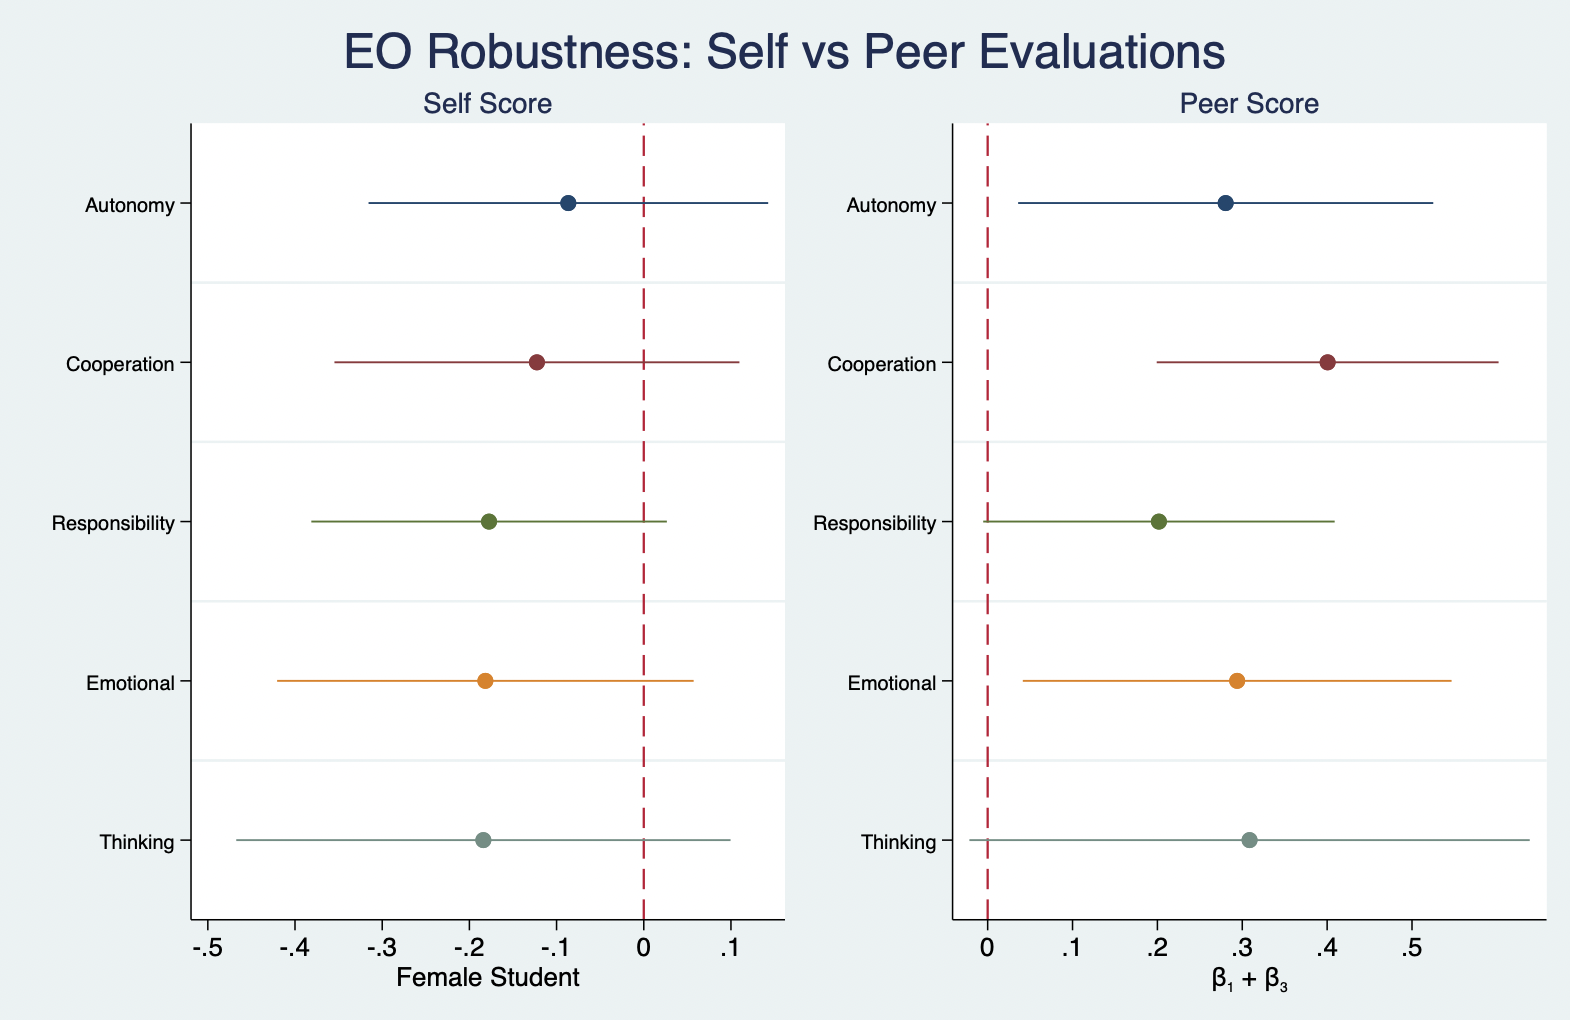
\includegraphics[width=0.75\textwidth]{figures/PB_self_peer_EO_combined.png}
\end{frame}

% ---- FA Robustness ----
\begin{frame}{Robustness: Lab-in-the-Field}
\label{slide:rob_fa}
\centering
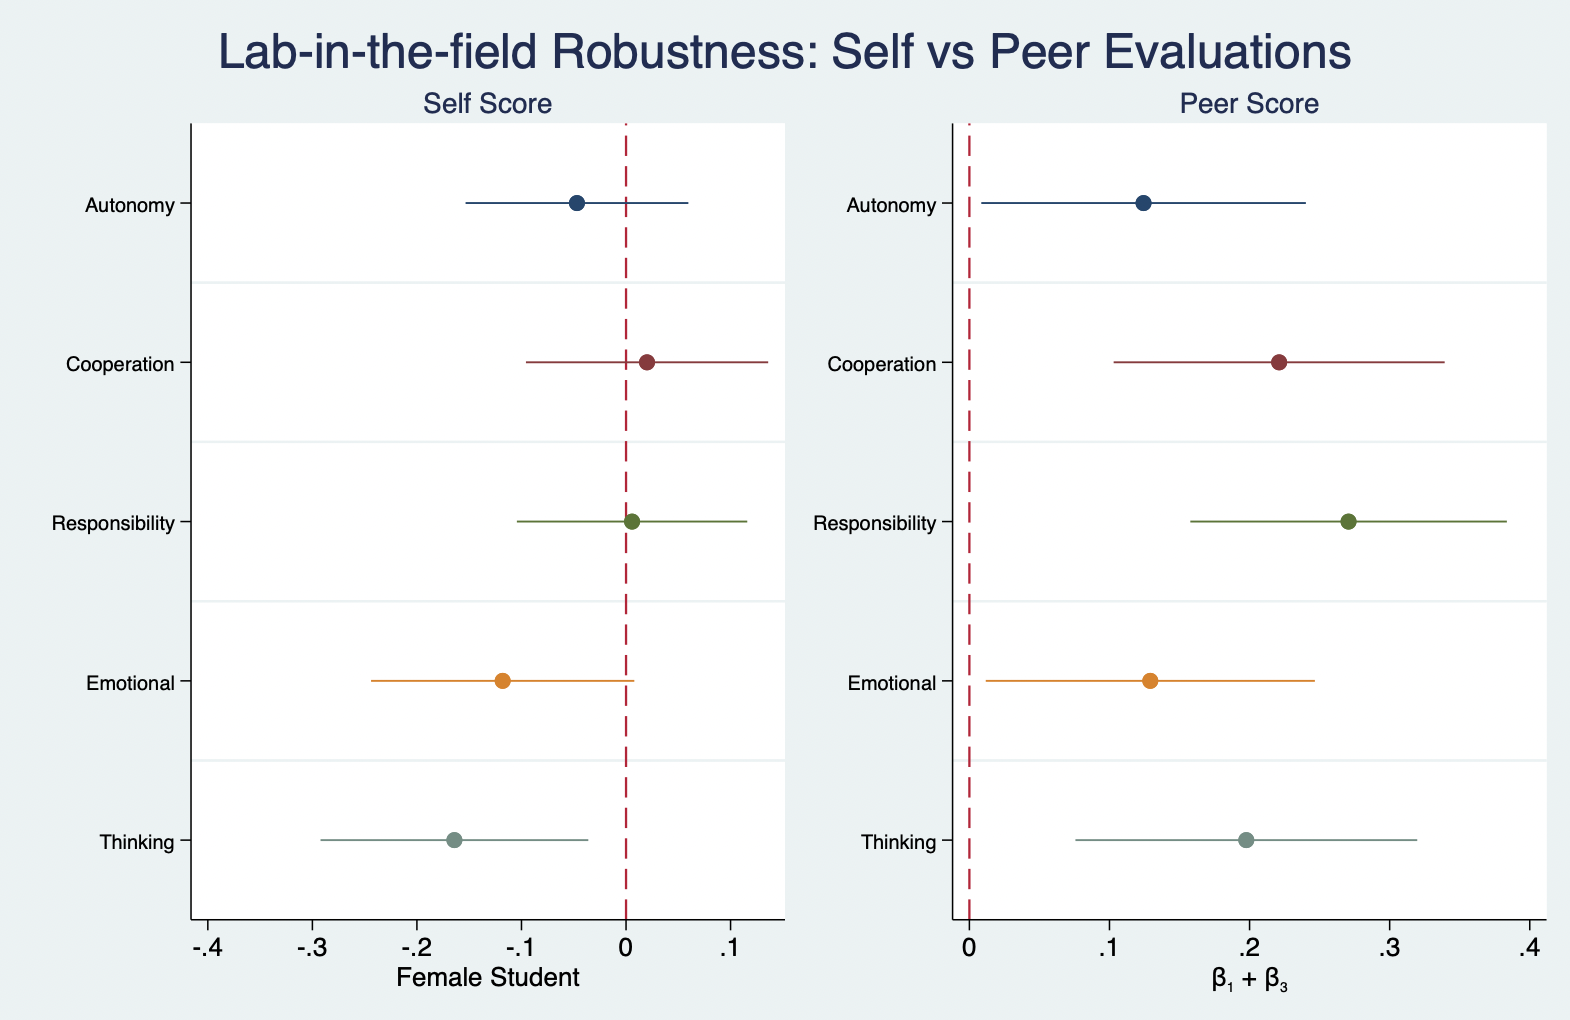
\includegraphics[width=0.75\textwidth]{figures/PB_self_peer_FA_combined.png}
\end{frame}

% ---- BESSI Robustness ----
\begin{frame}{Robustness: BESSI}
\label{slide:rob_bessi}
\centering
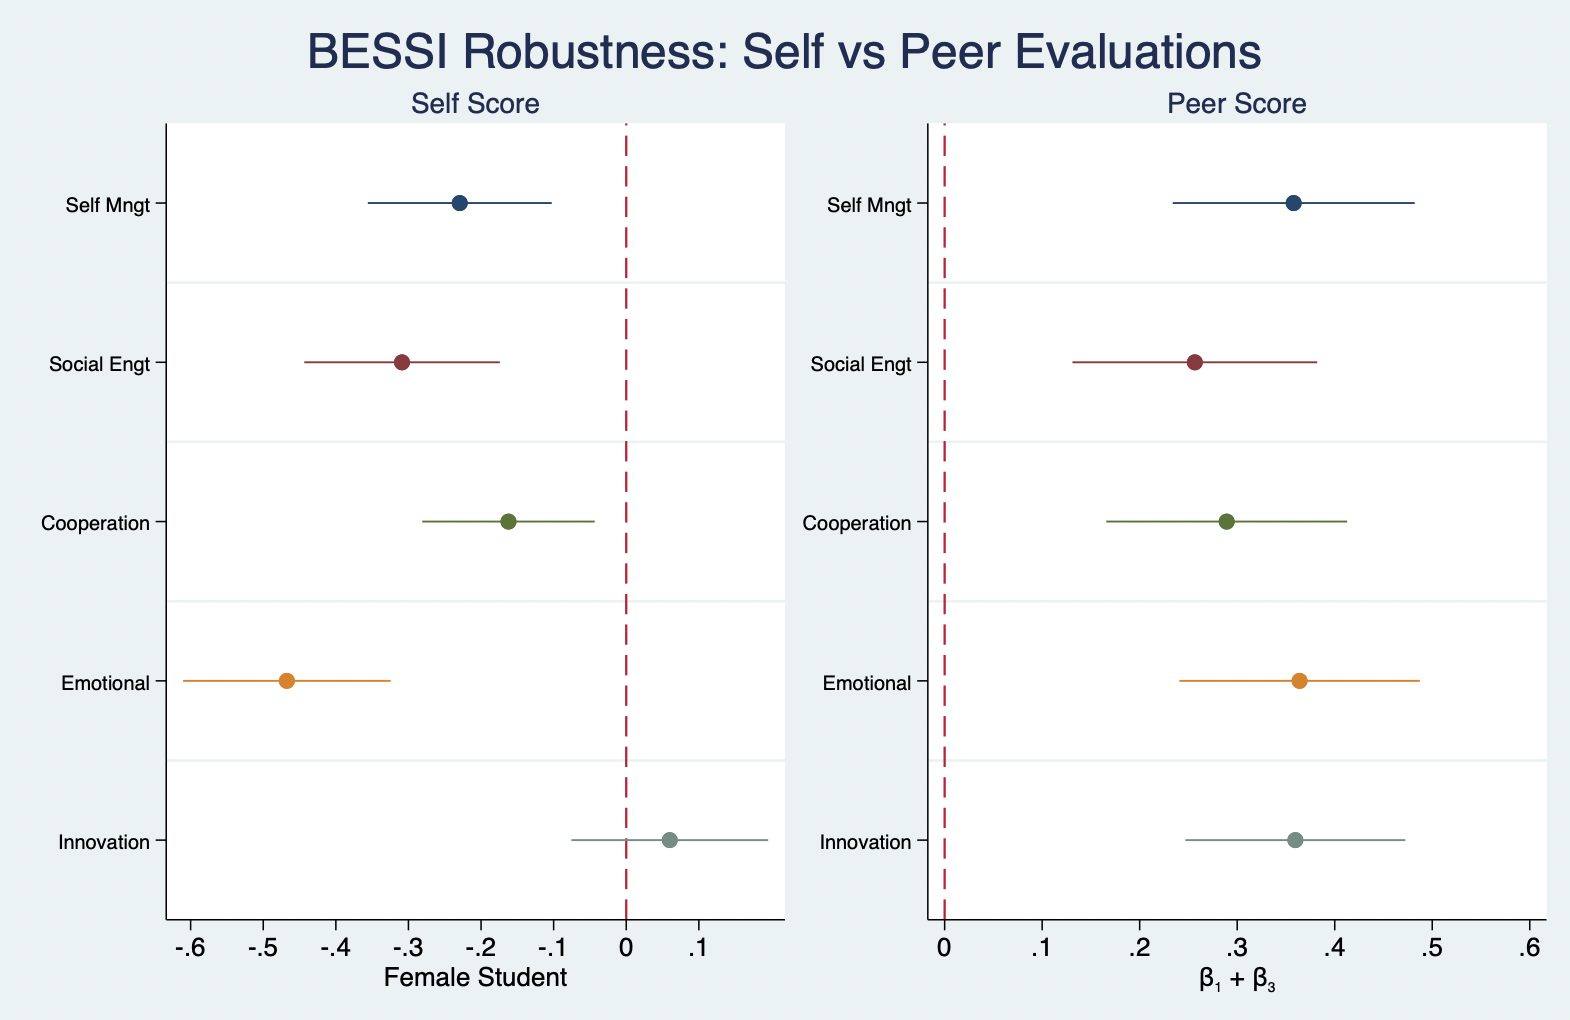
\includegraphics[width=0.75\textwidth]{figures/BESSI_self_peer_combined.png}
\end{frame}


% ---- Friendship Mediation (NEW since submitted version) ----
\begin{frame}{Friendship Mediation}
\label{slide:friendship}
\small
\pill{New since submitted version}

\vspace{0.3cm}
%TODO: Uncomment once friendship_combined_360.tex is generated
%
\begin{table}[htp]
\centering
\small
\begin{threeparttable}
\caption{Friendship Mediation of the Female-Female Premium}
\label{tab:friendship_combined}
\begin{tabular}{lccccc}
\toprule
 & Autonomy & Cooperation & Responsibility & Emotion & Thinking \\
\midrule
\multicolumn{6}{l}{\textit{Panel A: Classroom Observations}} \\[2pt]
Fem Stu $\times$ Fem Peer ($\beta_3$) & 0.374*** & 0.366*** & 0.139 & 0.251*** & 0.370*** \\
 & (0.097) & (0.078) & (0.085) & (0.087) & (0.088) \\
Obs$\rightarrow$Friend (BL) & 0.146*** & 0.117*** & 0.171*** & 0.203*** & 0.174*** \\
 & (0.050) & (0.043) & (0.042) & (0.045) & (0.047) \\[4pt]
$\beta_1 + \beta_3$ & 0.319*** & 0.281*** & 0.188*** & 0.252*** & 0.280*** \\
 & (0.074) & (0.059) & (0.065) & (0.070) & (0.076) \\
\% mediated &  19\% &  19\% &  19\% &  19\% &  19\% \\
Observations & 1626 & 2306 & 2224 & 1866 & 1718 \\
R-squared & 0.311 & 0.298 & 0.269 & 0.255 & 0.316 \\
\midrule
\multicolumn{6}{l}{\textit{Panel B: Lab-in-the-Field}} \\[2pt]
Fem Stu $\times$ Fem Peer ($\beta_3$) & 0.187** & 0.261*** & 0.243*** & 0.157* & 0.305*** \\
 & (0.089) & (0.089) & (0.084) & (0.095) & (0.095) \\
Obs$\rightarrow$Friend (BL) & 0.002 & -0.085* & -0.022 & -0.093* & -0.014 \\
 & (0.051) & (0.050) & (0.049) & (0.055) & (0.052) \\[4pt]
$\beta_1 + \beta_3$ & 0.170*** & 0.285*** & 0.311*** & 0.186*** & 0.256*** \\
 & (0.066) & (0.068) & (0.063) & (0.068) & (0.071) \\
\% mediated & 0\% & -11\% & -2\% & -20\% & -2\% \\
Observations & 1623 & 1619 & 1619 & 1592 & 1604 \\
R-squared & 0.345 & 0.373 & 0.370 & 0.287 & 0.316 \\
\midrule
 & Self Mngt & Social Engt & Cooperation & Emot. Mngt & Innovation \\
\midrule
\multicolumn{6}{l}{\textit{Panel C: BESSI}} \\[2pt]
Fem Stu $\times$ Fem Peer ($\beta_3$) & 0.268*** & 0.218** & 0.161* & 0.251*** & 0.160* \\
 & (0.086) & (0.098) & (0.092) & (0.089) & (0.084) \\
Obs$\rightarrow$Friend (BL) & 0.148*** & 0.126** & 0.168*** & 0.100* & 0.135*** \\
 & (0.054) & (0.054) & (0.053) & (0.053) & (0.051) \\[4pt]
$\beta_1 + \beta_3$ & 0.357*** & 0.226*** & 0.252*** & 0.355*** & 0.331*** \\
 & (0.070) & (0.072) & (0.069) & (0.070) & (0.063) \\
\% mediated & 11\% & 14\% & 16\% & 8\% & 11\% \\
Observations & 1106 & 1104 & 1103 & 1102 & 1102 \\
Adj. R-squared & 0.404 & 0.247 & 0.283 & 0.238 & 0.329 \\
\bottomrule
\end{tabular}
\begin{tablenotes}[flushleft]
\footnotesize
\item \textit{Note:} Each panel augments the baseline peer-evaluation regression with a friendship indicator (whether the observer nominated the student as a top-5 friend at baseline). Panel~A: classroom observations with 360° controls (teacher, self, peer-self, and peer-teacher scores). Panel~B: lab-in-the-field with EO and self score controls. Panel~C: BESSI endline peer evaluations with self and teacher score controls. All models include Female Student ($\beta_1$), Female Peer ($\beta_2$), student and peer background controls, and classroom fixed effects. SE clustered at student level. $\beta_1 + \beta_3$ is the net female--female effect. \% mediated $= 100 \times [1 - (\beta_1+\beta_3)^{\text{friend}}/(\beta_1+\beta_3)^{\text{base}}]$, where the base model excludes the friendship control. *$p<0.10$, **$p<0.05$, ***$p<0.01$.
\end{tablenotes}
\end{threeparttable}
\end{table}


\textcolor{gray}{\textit{[Table: $\beta_3$, friendship coeff., lincom, \% mediated across CO/FA/BESSI]}}

\vspace{0.3cm}
\textbf{Key result:} Friendship absorbs at most 19\% (CO), 8--16\% (BESSI), 0\% (FA) of the FF premium

\vspace{0.2cm}
Friendship predicts higher ratings ($\gamma \approx 0.15$ SD, significant), but enters \emph{additively} --- same boost for all pairings. Cannot explain a gender-specific pattern.
\end{frame}

% ---- Friendship Coefplot (NEW since submitted version) ----
\begin{frame}{Friendship \& Male Neutrality}
\label{slide:friendship_coef}
\small
\pill{New since submitted version}

\vspace{0.3cm}
%TODO: Uncomment once defense_friendship_coefplot.pdf is generated
%\centering
%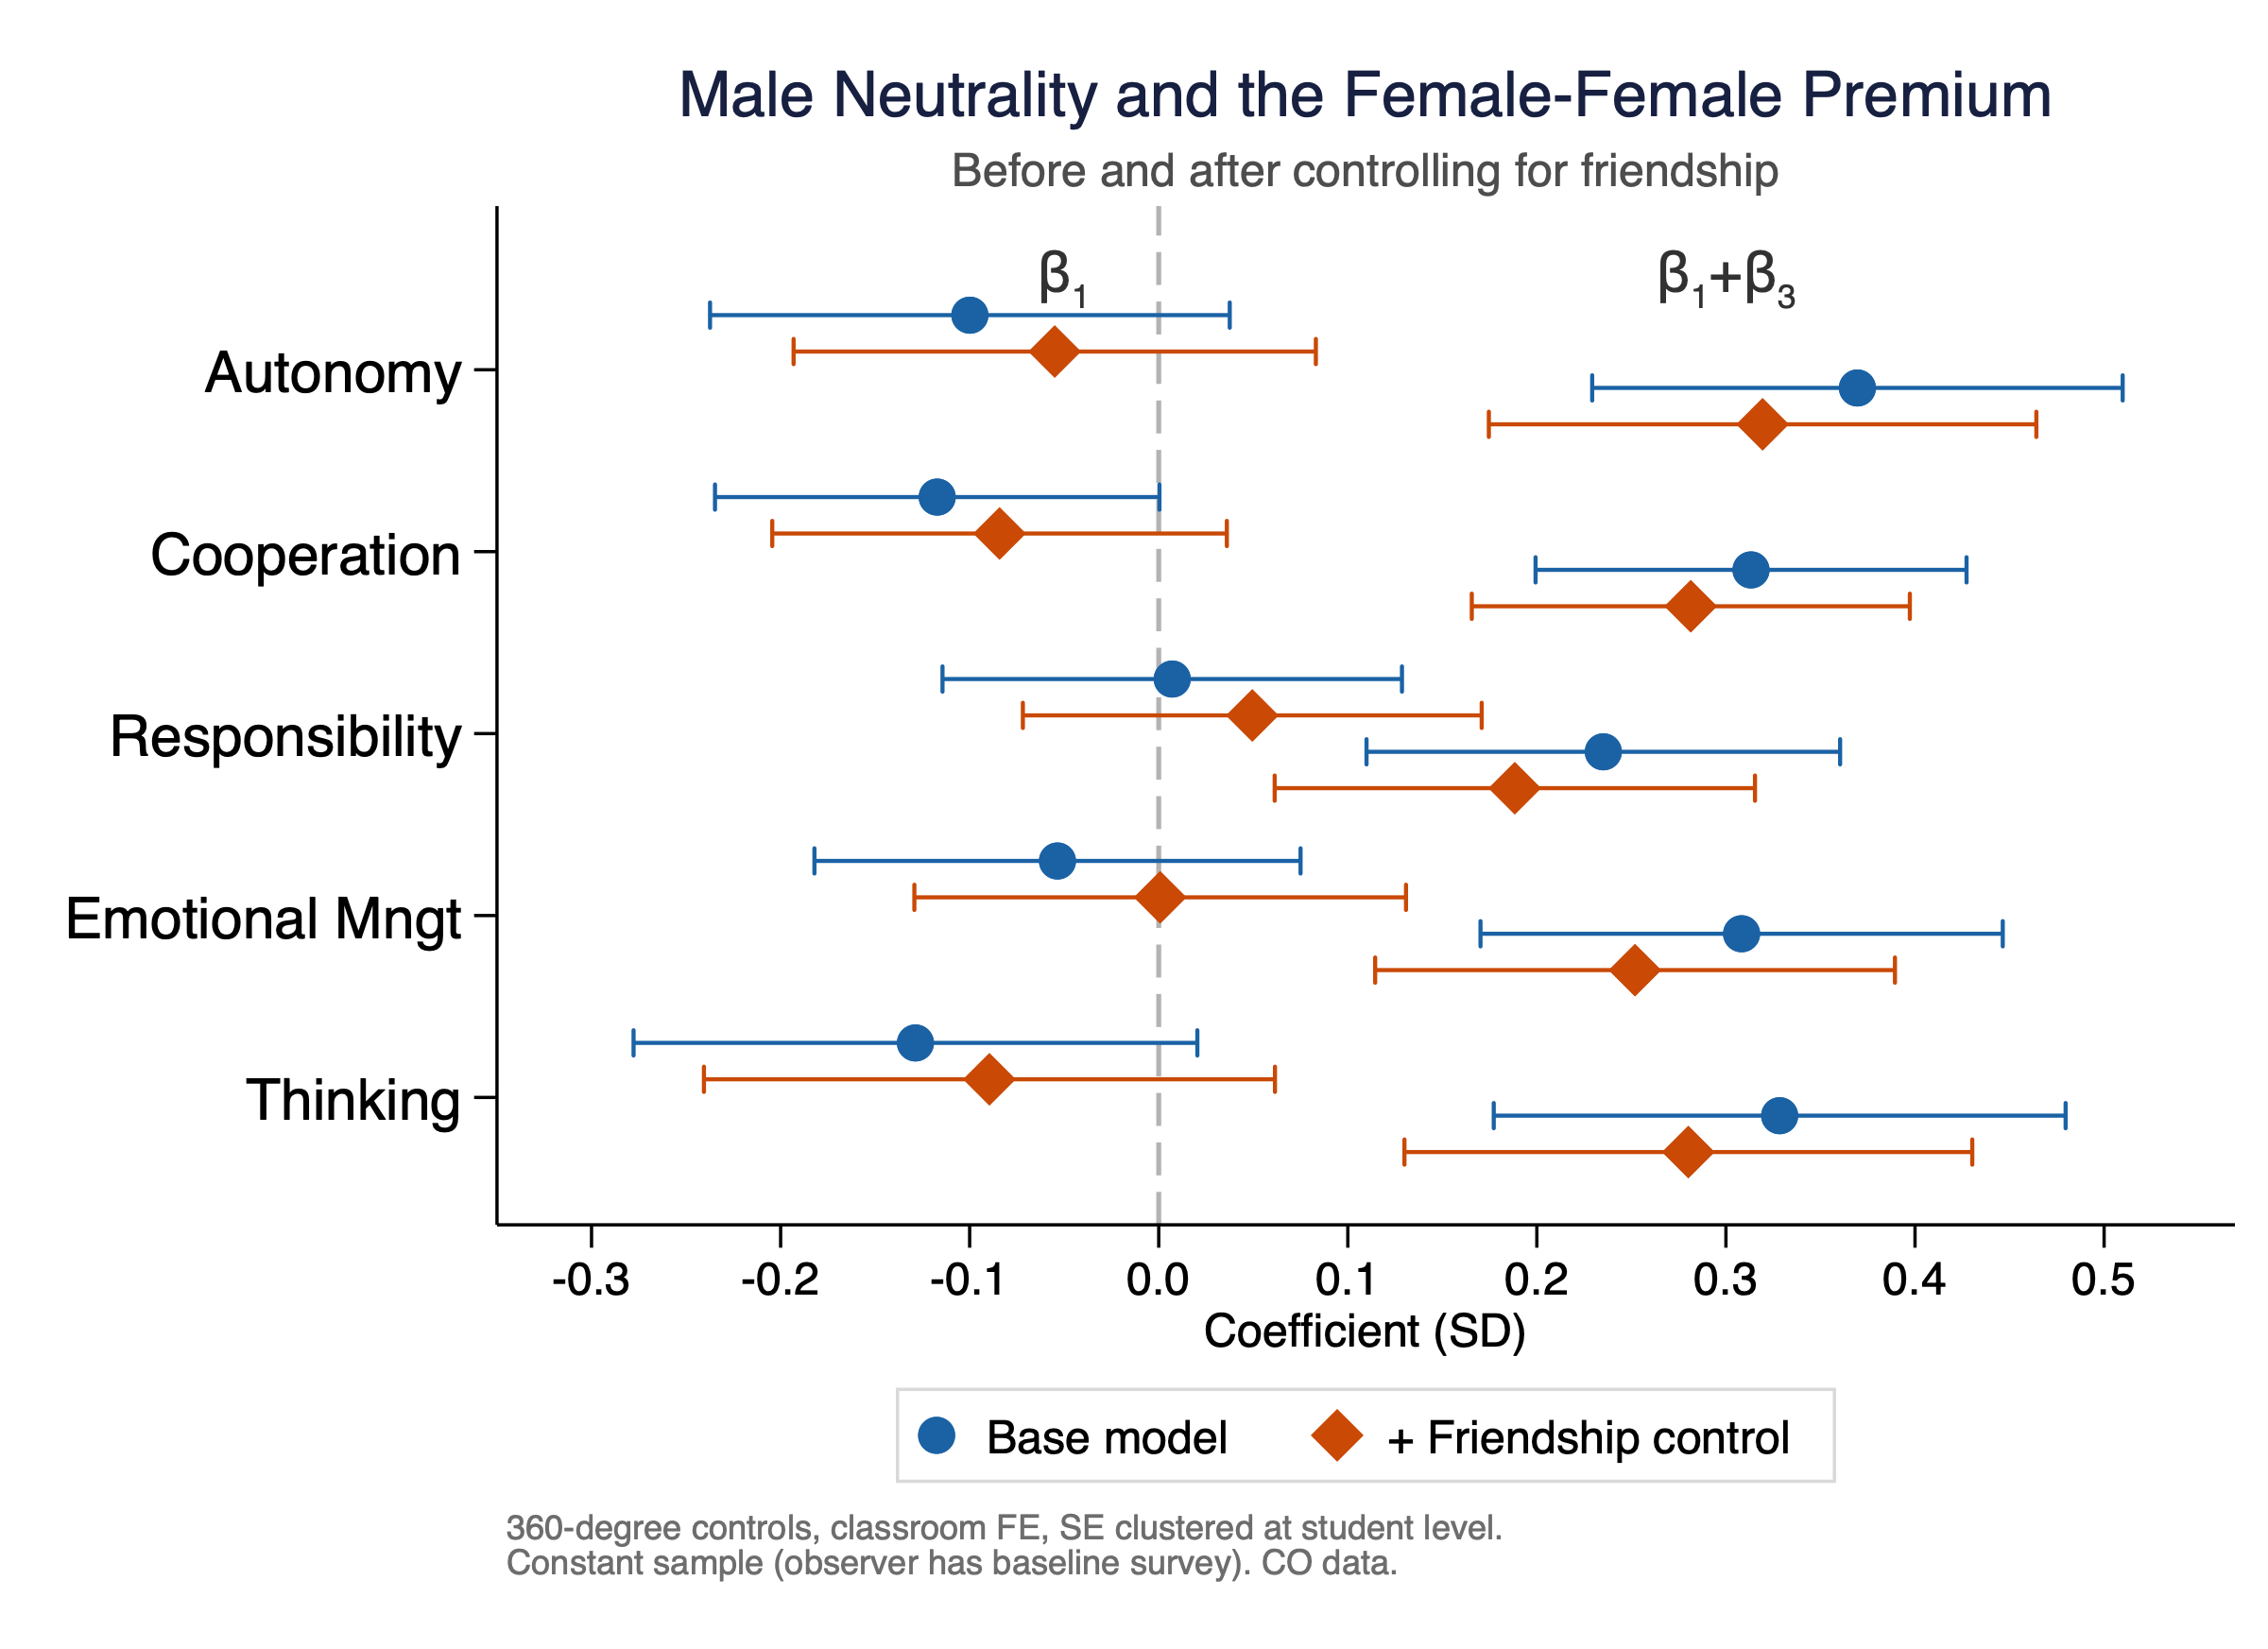
\includegraphics[width=0.8\textwidth]{figures/defense_friendship_coefplot.pdf}

\textcolor{gray}{\textit{[Figure: Horizontal coefplot --- $\beta_1$ and $\beta_1+\beta_3$ before/after friendship control]}}

\vspace{0.3cm}
\textbf{Reading the figure:}
\begin{itemize}
    \item Left cluster: $\beta_1 \approx 0$ in both models --- male peers are gender-neutral
    \item Right cluster: FF premium ($\beta_1 + \beta_3$) barely shifts with friendship --- only 10--20\% mediated
\end{itemize}
\end{frame}


% ---- Self-Evaluation Deviation (NEW since submitted version) ----
\begin{frame}{Self-Evaluation Deviations}
\label{slide:selfeval_dev}
\small
\pill{New since submitted version}

\vspace{0.3cm}
%TODO: Uncomment once figures are generated
%\includegraphics[width=0.8\textwidth]{figures/desc_selfeval_dev.png}

\textcolor{gray}{\textit{[Figures: Self minus benchmark gaps by gender (3 CO raw, 2 BESSI, 2 FA)]}}

\vspace{0.3cm}
\textbf{CO:} Males overestimate (+0.26 to +0.38 rubric points above peer ratings), females approximately calibrated

\vspace{0.2cm}
\textbf{BESSI/FA:} Genuine female underestimation
\end{frame}


% ---- Sample Attrition Funnel ----
\begin{frame}{Sample Attrition Funnel}
\label{slide:attrition}
\scriptsize
\begin{center}
\begin{tabular}{clc}
\toprule
Stage & What happens & Approx.\ $N$ \\
\midrule
0 & Raw universe & $\sim$3,648 \\
1--2 & Non-research removal, out-of-research grades & --- \\
3 & Consent ($\sim$66\% parental consent) & $\sim$2,680 \\
4 & Survey logistics (148 of 195 classrooms) & $\sim$2,451 \\
5 & Post-randomization attrition (5 classrooms) & $\sim$2,364 \\
6a & Ch.1 (RCT): regression-specific & 1,092--1,892 \\
6b & Ch.2 (Gender, CO): T only by design & 1,102 \\
6c & Ch.3 (FA/BESSI): T + C retained & 2,100--2,364 \\
\bottomrule
\end{tabular}
\end{center}

\vspace{0.2cm}
\footnotesize
\begin{itemize}
    \item Largest drop is consent ($\sim$34\%) --- standard for school-based RCTs in Spain
    \item 2,680 $\rightarrow$ 2,451 is survey logistics, not attrition (GESOP budget constraints)
    \item Ch.2 $N$=1,102 is smaller \emph{by design}: peer assessments only in treated classrooms
\end{itemize}
\end{frame}


% ---- Balance Tables ----
\begin{frame}{Balance Tables}
\label{slide:balance}
%TODO: \input{tables/balance_table}
\textcolor{gray}{\textit{[Balance table: student, school characteristics across T and C]}}
\end{frame}


% ---- Immigration Heterogeneity ----
\begin{frame}{Self-Evaluation Heterogeneity: Immigration}
\label{slide:immig_het}
\small
\pill{New since submitted version}

\vspace{0.3cm}
%TODO: \input{tables/mechanism/selfeval_het_immig}
\textcolor{gray}{\textit{[Table: Immigration is the only moderator with consistent heterogeneity]}}

\vspace{0.3cm}
Immigration widens the female self-evaluation gap in:
\begin{itemize}
    \item Cooperation (CO $-$0.280\sym{*}, BESSI $-$0.279\sym{**})
    \item Responsibility (CO $-$0.350\sym{**})
\end{itemize}
Other moderators (mother's education, SES index, school complexity) show no systematic pattern.
\end{frame}


% ---- Consequences Analysis ----
\begin{frame}{Self-Evaluation Consequences}
\label{slide:consequences}
\small
\pill{New since submitted version}

\vspace{0.3cm}
%TODO: \input{tables/mechanism/selfeval_consequences_gpa}
\textcolor{gray}{\textit{[Tables: GPA and absences as outcomes of self-evaluation gaps]}}

\vspace{0.3cm}
Correlational evidence on whether self-evaluation gaps predict GPA and absences.
\end{frame}


\end{document}
